%!TEX root = ../dokumentation.tex

\chapter{Hauptteil}
\label{cha:Hauptteil}

\section{Analyse}{
\label{sec:analyse}
In diesem Abschnitt werden die Anwendungsfälle nicht funktionalen Anforderungen dargestellt der zu entwickelnden Software zusammengefasst.
\subsection{Anwendungsfälle}{
Die verschiedenen Anwendungsfälle für die zu entwickelnde Grafische Oberfläche werden in diesem Abschnitt erläutert.

\subsubsection{Profil importieren}{
Der Kunde soll in der Lage sein, ein Profil in seinem Datenspeicher über die Menüführung der Workbench for Mill Plus auszuwählen. Das ausgewählte Profil soll in der Workbench geöffnet und in einem neuen Editor zur weiteren Bearbeitung angezeigt werden.
}

\subsubsection{Profil aktualisieren}{
Ist ein Profil im Editor der Workbench for Mill Plus geöffnet, soll es dem Anwender über verschiedene Methoden der Benutzerführung ermöglicht werden, die Aktualisierung des Profils zu starten. Ist das Profil zum aktuellen XML-Schema valide, soll keine Aktualisierung durchgeführt werden.
}

\subsubsection{Importiertes Profil verwenden}{
Ein importiertes Profil soll nach seinem Import in der \ac{DBWB} im Workflow des Benutzers  verwendet werden können. 
}

\subsubsection{Erzeugtes Profil verwenden}{
Ein vom Aktualisierungsvorgang erzeugtes Profil soll nach seiner Erstellung in der \ac{DBWB} im Workflow des Benutzers zur Filterkonfiguration verwendet werden können. 
}



}
\subsection{Nicht funktionale Anforderungen}{
Nicht funktionale Anforderungen sind Anforderungen, an die "Qualität" in welcher die geforderte Funktionalität zu erbringen ist. In diesem Abschnitt werden die nicht funktionalen Anforderungen erklärt.

\subsubsection{Handhabung}{
Bei den Anwendern der \ac{DBWB} handelt es sich meist um Personen, die im Dokumentmanagement tätig sind. Von Ihnen kann kein programmiertechnisches Expertenwissen erwartet werden, da dies nicht zum Schwerpunkt ihrer beruflichen Aufgaben gehört. Somit ist es erforderlich, die Funktionalität zur Aktualisierung von Profilen möglichst intuitiv in den bestehenden Workflow zu integrieren.
}
\subsubsection{Wartbarkeit}{
Die einzelnen \ac{OSGi}-Bundles sowie deren Zusammenspiel müssen einfach wartbar
sein, damit sie bei der Integration in das bestehende Produkt keine Mehrarbeit verursachen können. Auch für Updates und zukünftige Entwicklungen ist eine gute Wartbarkeit von großer Bedeutung. Ist eine Software schlecht wartbar, lassen sich neue oder geänderte Anforderungen meist nur mit hohem Aufwand umsetzen.
}
\subsubsection{Portierbarkeit}{
Das zu entwickelnde Plug-in soll auf allen Systemen verfügbar sein, auf denen auch die \ac{DBWB} ausgeliefert wird. Die Portierbarkeit bei modular aufgebauten Systemen hat eine große Bedeutung. Wird ihr wenig Aufmerksamkeit geschenkt, kann es sein, dass das entwickelte System nicht auf allen Zielplattformen das gleiche Verhalten aufweist.
}

\subsubsection{Konsistenz}{
Die Erweiterungen der \ac{DBWB} sollen eine Konsistenz in der Benutzerführung aufweisen. Zusätzliche Module und Plug-ins sollen nahtlos in den bestehenden Arbeitsablauf integriert werden, um die gewohnte Benutzbarkeit für den Anwender zu gewährleisten.
}


}

}

\section{Konzept}{
\label{sec:konzept}
In diesem Abschnitt wird das, dem zu entwickelnden Plug-in zugrundeliegende, Konzept erläutert.

\subsection{Grafische Einbettung}{
Die neu bereitgestellten Funktionalitäten sollen sich nahtlos in die bestehende Anwendung DocBridge\textsuperscript{\textregistered} Workbench for Mill integrieren. Darüber hinaus soll die grafische Einbettung den Standards der Compart AG für \ac{GUI}s genügen. Hierzu wurden die Benutzeroberfläche der \ac{DBWB} und firmeninterne Designvorlagen untersucht. Um eine hohe Benutzbarkeit zu gewährleisten werden dem Anwender mehrere Möglichkeiten gegeben, auf die hinzugefügten Funktionalitäten zuzugreifen. Um die grafische Einbindung zu visualisieren und zu veranschaulichen wurden \glspl{Mockup}, funktionsunfähige Modelle, angefertigt.
}

\subsection{Prototyp}{
Um die in den Anforderungen geforderten Funktionalitäten herzustellen werden diese erst in einem Prototypen simuliert. Dieser beinhaltet eine Komponente zum importieren und eine Komponente zum aktualisieren von Filterprofilen. Der Prototyp konzentriert sich bei der Aktualisierungskomponente zunächst auf den Dokumenttyp \ac{AFP}. 


\subsubsection{Komponente für den Profilimport}{
\label{sec:komp_profilimport}
Filterprofile werden in der \ac{DBWB} in einem Profile Repository verwaltet. Für gewöhnlich wird mit jeder neuen Version eines XML-Schemas ein default-Profil mitgeliefert, anhand dessen Vorlage sich der Anwender ein eigenes Profil erstellen lassen kann. Das erstellte Filterprofil kann beliebig modifiziert werden. Das default-Profil ist nicht zur Modifikation vorgesehen. Die Komponente liest aus dem importierten Profil die Version aus. Die Version ist in jedem Profil als Attribut abgelegt. Anhand der Version und einem eindeutigen Identifier wird eine neue Version im Profile Repository angelegt. Das Profil wird als neues default-Profil dieser Version abgelegt. Das hat den Vorteil, dass der Anwender sein importiertes Profil in der Dokumentenperspektive der \ac{DBWB} untersuchen, jedoch nicht verändern kann. Soll das importierte Profil modifiziert werden, muss der Benutzer anhand des neuen default-Profils ein neues Profil generieren lassen. Große Bedeutung kommt auch der Benutzerführung zu. In jeder der beiden Perspektiven der \ac{DBWB} ist der Import auf unterschiedliche Art und Weise zu handhaben. 


\textbf{Prozessperspektive}
 {
 
Dem Anwender steht in dieser Perspektive eine Projektnavigation zur Verfügung. Er soll beim Import eine Auswahlmöglichkeit für das Zielprojekt haben. Importierte Profile werden in einem Unterordner \texttt{profiles} im ausgewählten Projekt abgelegt. Anfangs war es vorgesehen, in der Prozessperspektive mehrere Filterprofile gleichzeitig importieren zu können. Während der Implementierung der Importkomponente wurde klar, dass dies der Konsistenz und Nutzerführung nicht zuträglich ist. Die Funktionalität wurde deshalb auf den Import eines einzelnen Profils beschränkt. Nach dem Import wird das Profil im Profile Repository abgelegt und in einem Editor geöffnet. Existiert im Projektunterverzeichnis \texttt{profiles} bereits ein Profil für den entsprechenden Filtertyp soll der Nutzer die Möglichkeit haben, das existente Profil zu überschreiben, das zu importierende Profil umzubenennen oder seine Aktion abzubrechen. 

}


\textbf{Dokumentenperspektive} 
{

In der Dokumentenperspektive betrachtet der Benutzer oft nur ein einzelnes Dokument, das mit Hilfe verschiedener Filter konvertiert werden kann. Deshalb ist es unnötig mehrere Profile importieren zu können. Die Komponente zur Projektnavigation ist in dieser Perspektive ebenfalls deaktiviert. Somit soll es beim Import in der Dokumentenperspektive auch nicht möglich sein, ein Projekt auszuwählen, in dem das Profil gespeichert wird. Es wird nur im Profile Repository abgelegt und in einem Editor geöffnet.

}



}

\subsubsection{Komponente zur Aktualisierung von Profilen}{
Bei der Aktualisierung von Profilen soll ein bereits vorhandenes Plug-in verwendet werden, das die Funktionalität der Konvertierung von Profilen zur Verfügung stellt. Den Use Case zeigt Abbildung \ref{fig:UpdateProfile_UseCase}. Geplant ist, dass für jeden Filtertyp ein eigenes Plug-in erstellt wird. Diese werden bei Bedarf eingebunden. Wie auch bei der Importkomponente soll sich die Aktualisierungskomponente in den bestehenden Arbeitsfluss integrieren. Ist ein Filterprofil in einem Editor ausgewählt, hat der Anwender verschiedene Möglichkeiten den Konvertierungsprozess anzustoßen. Neben einem Eintrag im Hauptmenü soll die Aktion auch über eine \gls{Toolbar} und ein Kontextmenü verfügbar sein. Nach starten des Prozesses über eine der genannten Möglichkeiten wird das aktuell geöffnete Profil ermittelt. Anhand des root-Tags\footnote{Hauptelement in der Profildatei} wird der Filtertyp(z.B. \ac{AFP},\ac{PDF}) ermittelt. Anhand dieses Filtertyps wird das benötigte Konvertierungs-Plug-in festgestellt und dessen convert()-Methode mit dem ausgewählten Profil als Übergabeparameter gestartet. Sobald die Konvertierung abgeschlossen ist, wird dem Anwender das originale und das generierte Profil angezeigt, um weitere Modifikationen vornehmen zu können, wie im Sequenzdiagramm Abbildung \ref{fig:ConversionSequenz} dargestellt ist. 
In einem Vergleichseditor soll der Nutzer darüber entscheiden, welche Änderungen übernommen und welche verworfen werden sollen. Die nachfolgenden Unterabschnitte stellen drei Ansätze dar, wie ein solcher Vergleichseditor realisiert werden kann.


\begin{figure}[H] 
  \centering
     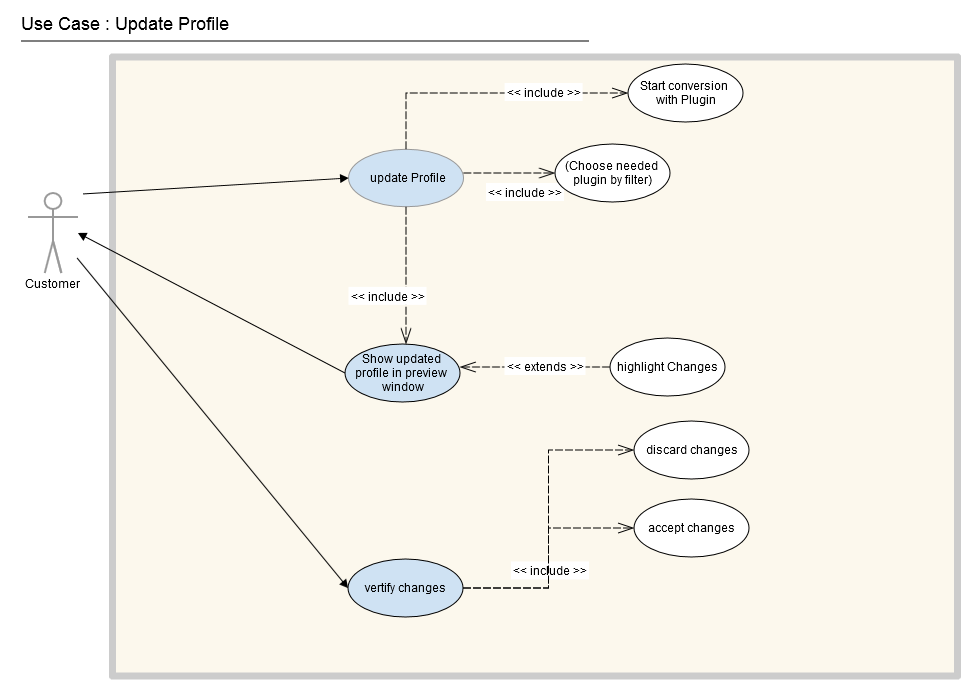
\includegraphics[height=.6\textwidth]{UpdateProfile_UseCase.png}
  \caption{Use Case Diagramm zum Aktualisieren der Profile}
  \label{fig:UpdateProfile_UseCase}
\end{figure}

\begin{figure}[H] 
  \centering
     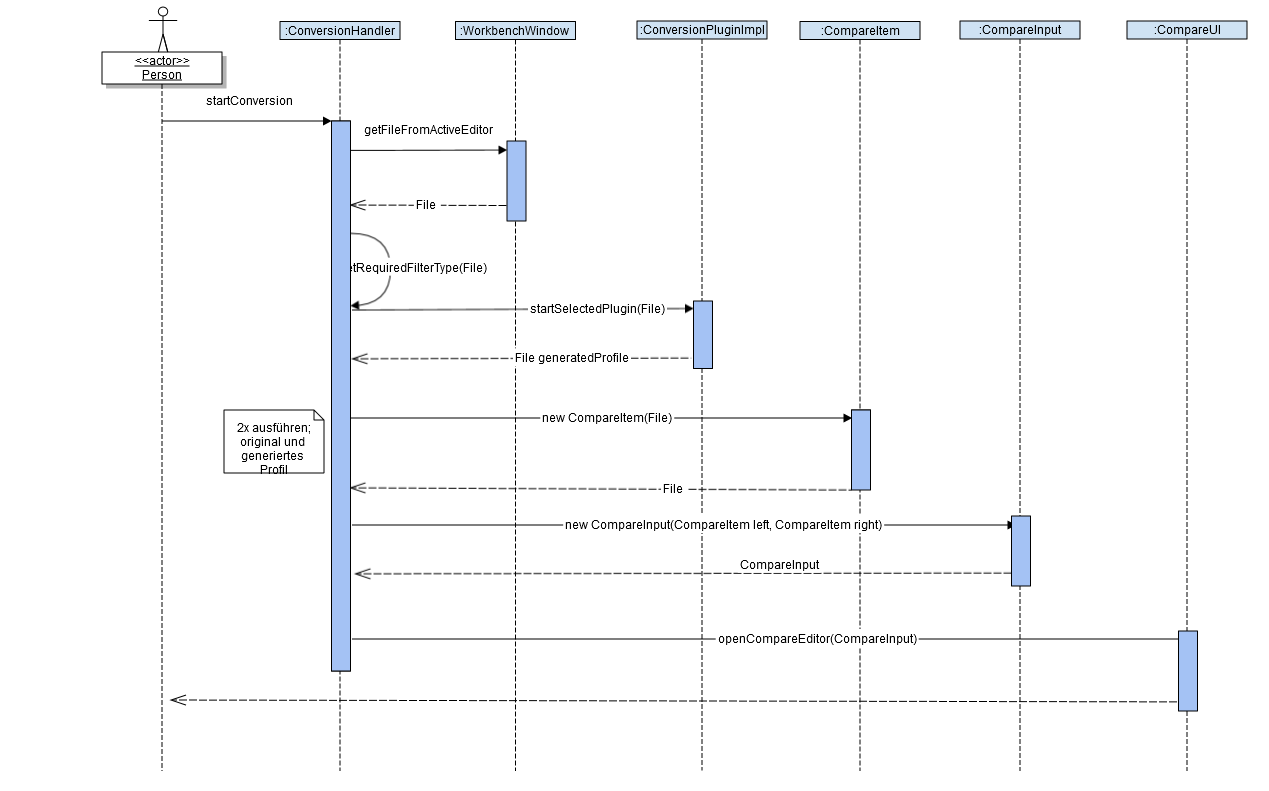
\includegraphics[height=.6\textwidth]{ConversionSequenz.png}
  \caption{Sequenzdiagramm zur Aktualisierungskomponente}
  \label{fig:ConversionSequenz}
\end{figure}






\textbf{Erweiterung des Dokumenteneditors}{

Der Editor der \ac{DBWB} ermöglicht es, eine Vorschau von zu konvertierenden Dokumenten anzuzeigen. Ist beispielsweise ein Dokument im \ac{AFP}-Format gegeben und soll nach \ac{PDF} konvertiert werden, so lässt sich das Ergebnis in einem Editor bereits zur Laufzeit betrachten. Geplant war das Überschreiben dieses Editors mit einem Standard XML-Editor. Dieser Ansatz musste verworfen werden, da dies im konzeptionellen Widerspruch zum etablierten Dokumenteneditor stand.

}

\textbf{Erstellen eines spezialisierten Editors}{

Der nächste Ansatz war es, einen Editor speziell zum Vergleich von zwei Filterprofildateien zu entwickeln. Ein EditorPart soll zwei weitere EditorParts enthalten, in denen das originale und das konvertierte Profil angezeigt werden. Eclipse \ac{RCP} sieht jedoch vor, dass ein Editor in Beziehung zu genau einer Datei steht. Deshalb musste dieser Ansatz ebenfalls verworfen werden. 

}

\textbf{Nutzung von CompareUI\footnote{Java \ac{API}
 um Vergleich von Objekten}}{
 
 Die Java Klasse \texttt{org.eclipse.compare.CompareUI} bietet einen Einstiegspunkt, um konfigurierbare Vergleichsoperationen auf beliebige Ressourcen durchzuführen. Das Ergebnis eines Vergleichs kann in einem speziellen Vergleichseditor geöffnet werden. Dieser Editor ermöglicht das dynamische Vergleichen einzelner Elemente von Dokumenten, was besonders am Beispiel von \ac{XML} oder \ac{HTML} ersichtlich wird. Auch das Eclipse Plug-in eGit\footnote{Plug-in zur grafischen Bedienung der Versionierungssoftware Git} nutzt die Klasse CompareUI, um Dateien in der Versionierungshistorie zu vergleichen. Ein solcher Vergleich ist in Abbildung \ref{fig:egit_compare} zu sehen. Da die Vorteile dieser Technologie nicht von der Hand zu weisen sind, wird dieser Ansatz zur Entwicklung zur Darstellung des Ergebnisses des Konvertierungs-Plug-ins gewählt.

\begin{figure}[htbp] 
  \centering
     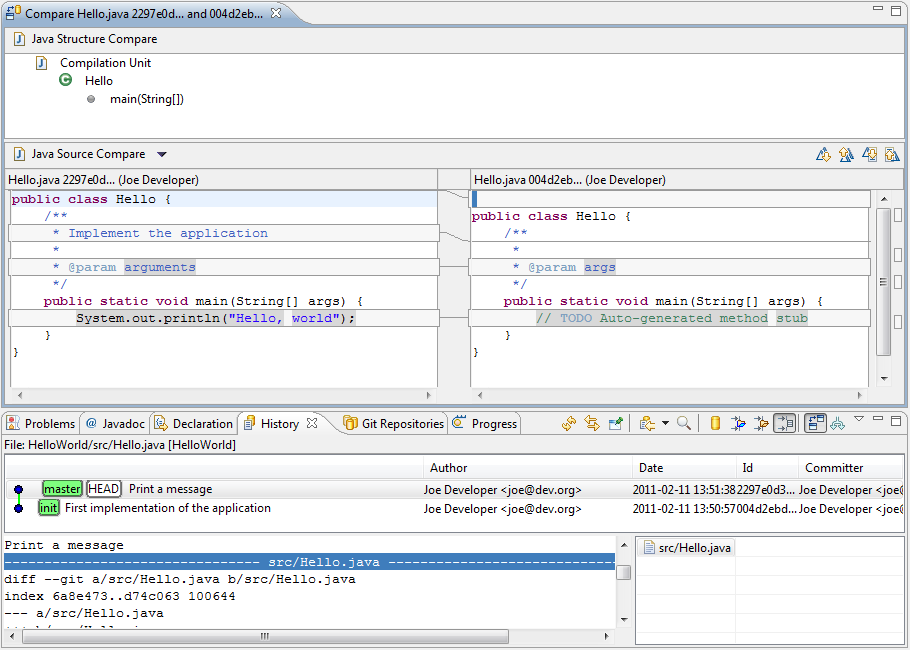
\includegraphics[height=.7\textwidth]{egit_compare.png}
  \caption{Verwendung der API CompareUI am Beispiel von eGit}
  \label{fig:egit_compare}
\end{figure}

}



}

}






\subsection{Design der Bundles}{
In der Softwareentwicklung ist die Unterteilung der Software in kleinere Einheiten vorteilhaft, da dies den Test, die Wartung und die Entwicklung allgemein vereinfacht.




}

\section{Implementierung}{
\label{sec:implementierung}
Dieser Abschnitt beschreibt die Implementierung der Komponenten für den Profilimport und die Aktualisierung der Filterprofile.

\subsection{Entwicklungsumgebung}{
Die Implementierung der Bundles erfolgt in der \ac{IDE} Eclipse\footnote{Version Kepler}. Da \ac{RCP} auf dem Eclipse-Framework basiert, liegt die Wahl dieser \ac{IDE} nahe. Für das Konfigurationsmanagement wird das Build-Management-Tool Apache Maven 2 verwendet, das in Abschnitt \ref{sec:apache_maven} beschrieben wird. Als Laufzeitumgebung wird die \ac{JRE}6 verwenden, da diese auch bei den bestehenden Bundles im Entwicklungsumfeld zum Einsatz kommt. Das Java-Projekt wird automatisiert täglich auf einem Jenkins\footnote{System zur kontinuierlichen Integration} System gebaut. Um die Codequalität des Projekts zu gewährleisten, wird Sonarqube\textsuperscript{\texttrademark} eingesetzt. Um eine gute, standardisierte Codequalität zu gewährleisten, wird SonarQube\textsuperscript{\texttrademark} eingesetzt (siehe Abschnitt \ref{sec:soanr_qube}). Zur \gls{Versionsverwaltung} wird die Versionierungssoftware Git, die ursprünglich für die Quellcode-Verwaltung des Linux-Kernels entwickelt wurde, genutzt. Die grafische Git-Repository-Management-Lösung Atlassian Stash ermöglicht ein übersichtliches Verwalten der genutzten \glspl{Repository}.
}




\subsection{Komponente für den Profilimport}{
\label{sec:impl_import}

\subsubsection{Extensions}{
Unter Verwendung des Extension-Point-Mechanismus von Eclipse \ac{RCP} wurden in der Plugin.xml des Bundles verschiedene Extensions angelegt.\\

\textbf{Grafische Steuerelemente}{

Für das ergänzen der Benutzeroberfläche der \ac {DBWB} wird der Extension-Point 

\texttt{org.eclipse.ui.menu} verwendet. Sowohl in der Toolbar der \ac{DBWB} als auch in ihrer Menüleiste werden Buttons bzw Menüeinträge hinzugefügt. Das aktivieren eines solchen Menüeintrags oder Buttons startet den in Abschnitt \ref{sec:impl_klassen} beschriebenen Handler. Listing \ref{lst:extension} zeigt den Einsatz einer Extension, um eine neue Menükontribution anzulegen.

}
\textbf{Handler}{

Neben den Extensions für die grafischen Steuerelemente wird eine Extension am Extension-Point \texttt{org.eclipse.ui.handlers} registriert. Dieser ImportHandler ist aktiv, falls in der Prozessperspektive ein Projekt selektiert ist, oder der Nutzer sich in der Dokumentenperspektive befindet (vgl. Abschnitt \ref{sec:komp_profilimport}). 
}

 \begin{lstlisting}[caption={Exemplarische Extension Points für Toolbareintrag und Importhandler},label=lst:extension]
/*
 * Extension Point fuer einen Toolbareintrag 
*/    
   <extension point="org.eclipse.ui.menus">
		<menuContribution
            allPopups="false"
            locationURI="toolbar:org.eclipse.ui.main.toolbar?
            after=net.compart.dbwb.filterconfigurator.
            documenteditor.exportProfilesButton">
         <toolbar
            id="net.compart.dbwb.filterconfigurator.toolbar">
            <command
                  commandId="com.compart.profileconverter.
                  ui.importmenu"
                  icon="icons/import_wiz.gif"
                  id="com.compart.profileconverter.ui.
                  importmenu.toolbar.main"
                  label="%importprofile.label"
                  style="push"
                  tooltip="%importprofile.tooltip">
            </command>
         </toolbar>
      </menuContribution>
      </extension>
/*
 * Extension Point fuer den Import Handler 
*/       
      <extension point="org.eclipse.ui.handlers">
            <handler
               class="com.compart.profileconverter.
               ui.importmenu.internal.ImportHandler"
               commandId="com.compart.profileconverter.
               ui.importmenu">
               <enabledWhen>
                 <or> 
                  <with
                        variable="selection">
                     <iterate
                           ifEmpty="false"
                           operator="or">
                        <instanceof
                            value="org.eclipse.core.
                            resources.IProject">
                        </instanceof>
                     </iterate>
                     <count  
                          value="1">  
                     </count>
                  </with>
                  <with variable="activeWorkbenchWindow.
                  activePerspective">
                      <equals
                          value="com.compart.dbwb.
                          productivitytools.
                          documentPerspective">
                      </equals>
                  </with>
                 </or>
               </enabledWhen>
            </handler>
      </extension>
 \end{lstlisting}


}

\subsubsection{Implementierte Klassen}{
\label{sec:impl_klassen}

In diesem Abschnitt werden die implementierten Klassen beschrieben. Das implementierte OSGi-Bundle verfügt nicht über eine Aktivator-Klasse, da der default Aktivator in unserem Falle ausreichend ist. Wie in \cite[S.70]{BertholdDaum} beschrieben kontrolliert die Aktivator-Klasse den Lebenszyklus des Plug-ins. Bei der Implementierung der Klassen wurden die in Tabelle \ref{tbl:extern_bibs} Bibliotheken verwendet.

\textbf{ImportHandler}{

In der von \texttt{org.eclipse.core.commands.AbstractHandler} abgeleiteten Klasse ImportHandler wird zunächst überprüft, in welcher Perspektive sich der Benutzer beim Aufruf befand. Handelt es sich um die Prozessperspektive, wird mit Hilfe eines Selection-Services, der in Listing \ref{lst:selectionService} abgebildet ist, das selektierte Projekt im Projektnavigator ermittelt. Ein FileDialog Widget \texttt{org.eclipse.swt.widgets.FileDialog} wird geöffnet, über den der Benutzer das zu importierende Profil auswählen kann. Existiert kein Filterprofil des gleichen Typs im Projekt, so wird die Datei im \texttt{profiles}-Unterverzeichnis des Projekts kopiert und mit Hilfe des ProfileRepositoryLocationProvider im ProfileRepository der \ac{DBWB} abgelegt. Existiert bereits ein Profil des gleichen Typs wird ein Dialog erzeugt, der dem Benutzer verschiedene Verfahrensmöglichkeiten bietet. Das im Projekt bestehende Profil kann überschrieben werden oder das zu importierende Profil kann umbenannt werden. Mit einem Enumerationsalgorithmus wird ein neuer Name erzeugt.

 \begin{lstlisting}[caption={Nutzung eines Selection Services, um das gewähle Projekt zu ermitteln},label=lst:selectionService]
  private IProject getSelectedProject()
          {
          IWorkbenchWindow window = 
          	this.page.getWorkbenchWindow();
          ISelection selection = 
          	window.getSelectionService().getSelection(PROJECT_NAV);
          if (!(selection instanceof IStructuredSelection))
              {
              return null;
              }
  
          Object o = 
          	((IStructuredSelection)selection).getFirstElement();
          IProject activeProject = (IProject)o;
          return activeProject;
          }
 \end{lstlisting}








}

\textbf{ProfileRepositoryLocationProvider}{

Der ProfileRepositoryLocationProvider wurde von einer in der \ac{DBWB} existierenden LocationProvider-Klasse abgeleitet. Dieser LocationProvider sucht nach, mit der DocBridge Mill Plus von Haus aus mitgelieferten, Filterprofilen und deren dazugehörigen XML-Schemata. Diese werden bereitgestellt und ins ProfileRepository kopiert. In der Klasse ProfileRepositoryLocationProvider werden viele Funktionen, die zur Ermittlung der Filterprofile dienen überschrieben, um eine eigene Profilversion zu erstellen. Ein Überladen des Konstruktors bietet die Möglichkeit, ein vom bestehenden System unabhängiges Profil einzubringen und ihm eine generierte Version zuzuordnen. Es wird eine eigene Location erstellt, mit der später das ProfileRepository aktualisiert werden kann. Listing \ref{lst:pushToRepo} zeigt den Aufruf des LocationProviders und die Aktualisierung des ProfileRepository.

 \begin{lstlisting}[caption={Methode, um Filterprofil im ProfileRepository abzulegen},label=lst:pushToRepo]
   
   private void pushfileToProfileRepository(File profile)
          {
          if (profile.exists() && profile.isFile())
              {
              ProfileRepositoryLocationProvider locationProvider = new ProfileRepositoryLocationProvider(profile);
              IRepository profileRepository = ProfileRepository.getProfileRepository();
              profileRepository.updateLocations(locationProvider);
              }
          }
 \end{lstlisting}


}
\textbf{Messages}{

Im Zusammenspiel mit verschiedenen Java-Properties-Dateien\footnote{Ein Java Konfigurationsmechanismus}, wird über die Klasse \texttt{Messages} die Lokalisierung der Nachrichten und Labels der \ac{RCP}-Applikation gesteuert. Dabei werden in der Klasse \texttt{Messages} alle benötigten \glspl{String} deklariert. Diese werden in Java-Properties-Dateien entsprechend mit der jeweiligen Lokalisierung definiert.

}

\subsection{Komponente zur Aktualisierung von Profilen}{
\label{sec:impl_aktualisieren}
Da der Aufgabenzeitraum für die Analyse, Konzeption und Implementierung beider Komponenten zu knapp bemessen war, konnte die Aktualisierungskomponente nicht vollständig implementiert werden. Es existiert jedoch ein Prototyp, der mit der Technologie CompareUI(Abbildung \ref{fig:egit_compare}), die bereits im \nameref{sec:konzept} erwähnt wird, realisiert wurde. Es wurde eine Standalone Eclipse \ac{RCP}-Anwendung implementiert, die über die Funktionalität verfügt, einen Vergleichseditor mit zwei Profilen zu öffnen. Da bereits ein detailliertes Konzept besteht, dürfte die Implementierung dieser Komponente nicht allzu Zeitaufwendig sein. Vor allem, da Sie sich nicht in großem Maß von der Programmierung der \nameref{sec:impl_import} unterscheidet.    

}

\subsection{Filterprofileditoren}{
Standardmäßig werden in der \ac{DBWB} die spezialisierten Editoren für Filterprofile anhand des Filtertyps gewählt. Ein \ac{AFP}-Profil wird beispielsweise mit einem speziellen Editor für \ac{AFP}-Profile geöffnet, der es dem Anwender ermöglicht, die Filterkonfiguration im Profil mit Hilfe einer grafischen Oberfläche vorzunehmen. In der Vergangenheit wurde der Dokumententyp des Profils anhand des Dateinamens ermittelt. Da mit dem Plug-in für den Profilimport dem Benutzer jedoch die Möglichkeit gegeben wird, importierte Profile in der Prozessperspektive umzubenennen(vgl. Abschnitt \ref{sec:impl_klassen}), musste eine Lösung gefunden werden, wie man Filterprofile anhand ihres Inhaltes einem Filtertyp zuordnen kann. Die Lösung fand sich in der Editierung der Plug-in-Manifest-Datei (plugin.xml). Statt den Dateinamen abzufragen wurde die Extension \texttt{org.eclipse.core.contenttype.contentTypes} überarbeitet und um einen Describer
\\
\texttt{org.eclipse.core.runtime.content.XMLRootElementContentDescriber} erweitert. Dieser erkennt das \ac{XML}-Root-Element\footnote{Äußerstes Element in einer XML-Datei} und ordnet anhand des erkannten Typs einen Profileditor zu.

\begin{lstlisting}[caption={Bearbeitete ContentType-Extension am Beispiel des Formattyps AFP},label=lst:filter_editor]
  <extension point="org.eclipse.core.contenttype.contentTypes">
        <content-type
              base-type="org.eclipse.core.runtime.xml"
              file-extensions="pro"
              id="net.compart.dbwb.filterconfigurator.mffprofile.afp"
              name="%contenttypes.mffprofile.afp.label"
              priority="high">
              <describer
                  class="org.eclipse.core.runtime.content.
                  XMLRootElementContentDescriber">
                        <parameter 
                                  name="element" 
                                  value="mffafp">
                        </parameter>
             </describer>
        </content-type>
   </extension>
\end{lstlisting}




}


\subsection{Logging}{
Um den Ablauf von komplexen Programmen im Nachhinein verstehen zu können ist das \glspl{Logging} von Programmzuständen ein wichtiger Teil der Softwareentwicklung. 
Im Softwareumfeld der \ac{DBWB} existiert ein Logging Interface, das für alle Erweiterungen der Workbench genutzt wird. So wird das Verschmutzen der Software mit unterschiedlichen Logging-Konfigurationen vermieden. Es stehen zwei Arten von Loggern zur Verfügung. Der ContextLogger wird mit der zu loggenden Klasse initialisiert. Alle Meldungen werden sowohl in die, für den Benutzer vorgesehene, Log-Datei geschrieben. Der ContextLogger protokolliert auch in ein Trace-File. Der TechnicalLogger dagegen protokolliert dagegen ausschließlich in das Trace-File, das vor allem dem Support bei der Fehlerfindung helfen soll. Das Logging an sich unterscheidet sich in \ac{OSGi}-Anwendungen nicht von dem in Standard Java Applikationen. Zwar bietet \ac{OSGi} einen eigenen Log-Service, dieser verhält sich jedoch äquivalent und arbeitet ebenfalls mit verschiedenen Log-Leveln. 

}



\subsection{Verwendete Bibliotheken}{
In diesem Unterabschnitt sind die verwendeten Java-Bibliotheken aufgelistet und kurz beschrieben.
\begin{table}[H]
    \begin{tabular}{|p{7cm}|p{7cm}|}
    \hline
    \textbf{Bibliothek}                        & \textbf{Funktion}                                                                                                                                                             \\ \hline
    Java.io                           & Stellt Funktionen für Ein-und Ausgabestreams zur Verfügung. Auch Operationen auf dem Dateisystem und zur Serialisierung stellen einen wichtigen Teil dieser API dar. \\ \hline
    java.util                         & Enthält das Collecion-Framework, Event Model, Zeit- und Datumsfunktionalitäten. Darüber hinaus bietet es viele Utility-Funktionen.                                   \\ \hline
    javax.xml.parsers                 & Stellt Parser zur Bearbeitung von XML-Dokumenten zur Verfügung. Folgende Parser werden Unterstützt: SAX (Simple API for XML), DOM (Document Object Model)         \\ \hline
    org.apache.commons.lang           & Bietet statische Utility-Klassen, wie beispielsweise zur String-Modellierung.                                                                                        \\ \hline
    org.w3c.dom                       & API des Document Object Models. Bietet Zugriff und Modifikationsmöglichkeiten auf Dokumente.                                                                         \\ \hline
    
    org.eclipse.osgi.util             & Stellt Funktionalitäten bereit, um OSGi-Ressourcen handzuhaben.                                                                                                      \\ \hline
    org.eclipse.ui                    & API mit der das Eclipse RCP Benutzerinterface erweitert werden kann.                                                                                                 \\ \hline
    org.eclipse.swt                   & Stellt die Funktionalitäten des Standard Widget Toolkits bereit.                                                                                                     \\ \hline
    org.eclipse.jface                 & Ergänzt SWT um MVC (Model-View-Controller)-Ansatz                                                                                                                     \\ \hline
    org.eclipse.core                  & Ermöglicht die Entwicklung von RCP-Komponenten im Zusammenspiel mit dem Dateisystem.                                                                                 \\ \hline
    \end{tabular}
    \caption {Verwendete externe Java-Bibliotheken}
    \label{tbl:extern_bibs}
\end{table}


}



}


\section{Ergebnisse}{
\label{sec:ergebnisse}
In diesem Abschnitt werden die Erkenntnisse und Ergebnisse dieser Arbeit dargestellt, zusammengefasst und bewertet.

\subsection{Zusammenfassung}{
\label{sec:zusammenfassung}
In dieser Arbeit stellte die Einarbeitung in verschiedene Technologien wie \ac{OSGi} oder das \ac{RCP}-Framework einen Schwerpunkt dar. Es wurde ein \ac{OSGi}-Bundle im \ac{RCP}-Umfeld entwickelt und implementiert, das den Anwendern der DocBridge\textsuperscript{\textregistered} Workbench for Mill Plus die Möglichkeit verleiht, Filterprofile zu importierten und diese für die Konfiguration der In-und Outputfilter zu verwenden.
Darüber hinaus wurde ein Konzept entwickelt, wie ein bestehendes Plug-in zur Konvertierung von Filterprofilen anhand eines gegebenen XML-Schemas, grafisch in die bestehende Oberfläche der \ac{DBWB} eingebunden werden kann. 
}


\subsection{Bewertung}{
\label{sec:bewertung}
Die implementierte Softwarelösung entspricht im allgemeinen den Anforderungen, die an dieses Projekt gestellt wurden. Das Plug-in für den Import von Filterprofilen ermöglicht es dem Benutzer der \ac{DBWB}, Profile von seinem Dateisystem zu importieren und durch das Ablegen der Dateien im ProfileRepository, diese für die Konfiguration der In-und Output-Filter zur Modifikation und Konvertierung von Dokumenten zu verwenden. Bei der Implementierung wurde darauf geachtet, dass die implementierte Lösung ein möglichst allgemeingültiges Verhalten aufweist. Das Plug-in beschränkt sich nicht auf einzelne Filtertypen, sondern deckt alle möglichen Formate ab. Auch die nicht funktionalen Anforderungen wurden erfüllt, da sich das Plug-in nahtlos in die bestehende Benutzeroberfläche einfügt. Somit behindert es den Nutzer nicht bei bereits bestehenden Arbeitsabläufen. Es erweitert die \ac{DBWB} lediglich um eine weitere Funktionalität. Im Rahmen dieser Arbeit, bot \ac{OSGi} ein ideales Werkzeug zur Erweiterung eines bestehenden, modularisierten Systems. Generell besteht bei der Anwendung einer Technologie Bedarf an Entwicklern mit Expertenwissen. Bei \ac{OSGi} verhält es sich auch so. Die nötige Einarbeitungszeit wurde Anfangs unterschätzt, jedoch stellte sich die Unterteilung einer Anwendung in einzelne Bundles als sehr nutzbringend heraus und trägt zur Erweiterbarkeit der Applikation bei. Eclipse \ac{RCP} stellt ein mächtiges \glspl{Framework} bereit, mit dem sich spezialisierte Applikationen mit relativ wenig Aufwand entwickeln lassen.
} 


}

\section{Ausblick}{
\label{sec:Ausblick}
Da sich in der Softwareentwicklung auch noch während der Implementierung die Projektanforderungen ändern können, spricht man oft davon, dass Software nie fertig wird. Auch bei dieser Arbeit stellte sich im Laufe der Entwicklung und Implementierung heraus, dass die Anforderungen im Nachhinein erweitert werden müssen. Zum jetzigen Zeitpunkt existiert keine Möglichkeit, default-Filterprofile aus dem ProfileRepository zu entfernen. Um das Profile Import Plug-in dem Endnutzer zur Verfügung zu stellen sollte jedoch eine solche Funktionalität implementiert werden, da sonst die Verwaltung der importierten Filterprofile zu unübersichtlich werden würde. Die Profile können momentan manuell vom Dateisystem und somit auch aus dem ProfileRepository gelöscht werden, jedoch entspricht dies nicht den Anforderungen an die Benutzbarkeit. Ein weiterer Punkt der in der Zukunft überarbeitet werden sollte ist das Umbenennen von Profilen beim Import in der Prozessperspektive. Da zusätzliche Profile des gleichen Typs aufsteigend nummeriert werden, kann dies zur Verwirrung des Anwenders führen. Besonders, wenn ein Profil mitten aus der Enumeration gelöscht und durch ein neueres ersetzt wird. Der Anwender soll in Zukunft seine Profile selbst benennen können. Aufgrund der Begrenzen Zeit des Projekts war es nicht möglich, Tests zu konzipieren und zu implementieren. Dies muss vor dem Praktischen Einsatz des Import-Plug-ins geschehen. Geplant sind GUI-Tests mit Jubula\footnote{Eclipsebasiertes Tool zum automatisierten Testen von grafischen Benutzeroberflächen} und Cross-Plattform-Tests\footnote{Tests auf verschiedenen Betriebssystemen z.B. Linux, Windows, Solaris}, da das Plug-in bisher ausschließlich auf Windows 64 Bit implementiert und getestet wurde.
}



}

